\documentclass[12pt, letter, oneside]{report}
\usepackage{tikz}
\usetikzlibrary{shapes, arrows, chains, positioning, calc}
\usepackage[noend]{algpseudocode}
\usepackage{afterpage}
\usepackage{pdflscape} % horizontal pages
\usepackage{array} % control the size of columns in tables
% \usepackage{rotating} % tables
\usepackage{algorithm}
\usepackage[spanish]{babel}
\usepackage[utf8x]{inputenc}
\usepackage[obeyspaces]{url}
\usepackage{graphicx,latexsym,amssymb,color}
\usepackage{subfig}
\usepackage{pdfpages} % include external files
\usepackage{enumerate}
%\usepackage{times}
\usepackage{titlesec}
\usepackage{titletoc}
\usepackage{setspace}
    \onehalfspacing %space between lines
\usepackage{todonotes}
\usepackage{multirow} % combine cells in tabular environment
\usepackage{amsmath} % multiline equation, split
\usepackage{minted} % fancy code hightlighting as Pygments
    \usemintedstyle{murphy}
    \renewcommand{\theFancyVerbLine}{
        \sffamily\textcolor[rgb]{0.1,0.1,0.1}{\scriptsize\arabic{FancyVerbLine}}
    }

% \usepackage[none]{hyphenat} % problems with hyphenation

% rules of code
\usepackage{listings}
\lstset{
    language=Matlab,
    basicstyle={\small\ttfamily},
    stringstyle=\color{gray},
    keywordstyle=\color{blue},
    numberstyle=\color{blue},
    numbers=left,
    frame=single, 
    % rulesepcolor=\color{gray},
    showstringspaces=false
}

% change the format of title chapters --> titlesec package
\titleformat{\chapter}[hang]
    {\selectfont\huge}
    {\chaptertitlename\ \Roman{chapter}.}
    {20pt}{\huge}

    % less space before chapter titles
    \titlespacing*{\chapter}{0pt}{-50pt}{40pt}

% change the format of table of contents --> titletoc
\renewcommand{\thechapter}{\Roman{chapter}}
\renewcommand\thesection{\arabic{chapter}.\arabic{section}}
\renewcommand\thesubsection{\thesection.\arabic{subsection}}
\titlecontents{chapter}
    [0pt]
    {\addvspace{1pt}} % space above the title
    {\chaptertitlename\ {\thecontentslabel}. }
    {}
    {} % title ........... page X
    [\addvspace{1pt}] % space below the title

% configure links
\usepackage[pagebackref, bookmarks = true]{hyperref}
\hypersetup{
    colorlinks,
    citecolor    = blue,
    pdfborder    = {0 0 0}, % this solution is temporal
}
\usepackage{bookmark}

% backreferences
\renewcommand*{\backreflastsep}{, }
\renewcommand*{\backreftwosep}{, }
\renewcommand*{\backref}[1]{}
\renewcommand*{\backrefalt}[4]{%
    \ifcase #1 %
        \relax % or 'No citations'
    \or
        (página #2). % page
    \else
        (páginas #2). % pages
    \fi
}

% change padding columns in tables
\renewcommand{\tabcolsep}{3.5mm}
% change padding rows in tables
\renewcommand{\arraystretch}{1.5}

% hack backref
% HACK TO RUN pagebackref 
% by cyberSingularity from tex.stackexchange.com

\newif\ifbackrefshowonlyfirst
\backrefshowonlyfirstfalse
%
% hyperref is essential for this patch to make any sense, so it is not
% unreasonable to request it be loaded before applying the patch
\makeatletter
% 1. insert a phantomsection before every cite, so hyperref has something to
% target * in case natbib is loaded. hyperref provides an appropriate hook so
% this should be safe, and we don't even need to check if natbib is loaded!

\let\BR@direct@old@hyper@natlinkstart\hyper@natlinkstart
\renewcommand*{\hyper@natlinkstart}{\phantomsection\BR@direct@old@hyper@natlinkstart}

% note that the anchor will appear after any brackets at the start of the
% citation, but that's not really a big issue?
%    * if natbib isn't used, backref lets \@citex to \BR@citex during
%    \AtBeginDocument so just patch \BR@citex

\let\BR@direct@oldBR@citex\BR@citex
\renewcommand*{\BR@citex}{\phantomsection\BR@direct@oldBR@citex}%

% 2. if using page numbers, show the page number but still hyperlink to the
% phantomsection instead of just the page!

\long\def\hyper@page@BR@direct@ref#1#2#3{\hyperlink{#3}{#1}}

% check which package option the user loaded (pages (hyperpageref) or sections
% (hyperref)?)
\ifx\backrefxxx\hyper@page@backref
% they wanted pages! make sure they get our re-definition
\let\backrefxxx\hyper@page@BR@direct@ref \ifbackrefshowonlyfirst
%\let\backrefxxxdupe\hyper@page@backref% test only the page number
\newcommand*{\backrefxxxdupe}[3]{#1}% test only the page number \fi \else
\ifbackrefshowonlyfirst \newcommand*{\backrefxxxdupe}[3]{#2}% test only the
section name \fi \fi

% 3. now make sure that even if there is no numbered section, the hyperref's
% still work instead of going to the start of the document!
\RequirePackage{etoolbox}
\patchcmd{\Hy@backout}{Doc-Start}{\@currentHref}{}{\errmessage{I can't seem to
patch backref}} \makeatother

%%%% END BACKREF HACK



% title page

% title page

\usepackage[a4paper, hmargin={2.5cm, 2.5cm}, vmargin={2.5cm, 2.5cm}]{geometry}
% apply margins to only one page

\newcommand*{\titleGP}{\begingroup 
\centering % Center all text
\thispagestyle{empty}

{\fontfamily{phv}\selectfont

    % Logo UJAT
    \begin{minipage}[ht]{0.14\textwidth}
        \flushleft
        
\includegraphics[width=2cm]{images/logo-ujat.eps}
    \end{minipage}
    % Name of the University
    \begin{minipage}[ht]{0.70\textwidth}
    \centering
    {\fontfamily{phv}\selectfont
    {\bfseries{\normalsize UNIVERSIDAD JUÁREZ AUTÓNOMA DE TABASCO}}\\
    {\bfseries{\normalsize DIVISIÓN ACADÉMICA DE INFORMÁTICA Y SISTEMAS}}}
    \end{minipage}
    % logo DAIS
    \begin{minipage}[ht]{0.14\textwidth}
        \flushright
        
\includegraphics[width=3cm]{images/logo-dais.eps}
    \end{minipage}

    \rule{\textwidth}{3pt}\vspace*{-\baselineskip}\vspace{7pt} 
    \rule{\textwidth}{4pt}\vspace*{-\baselineskip}\vspace{7pt} 
    \rule{\textwidth}{3pt}\\[\baselineskip] 
    
    % Vertical lines
    \begin{minipage}[ht]{0.10\textwidth}
        \flushleft
        \rule{3pt}{16cm} 
        \rule{4pt}{16cm} 
        \rule{3pt}{16cm} 
    \end{minipage}
    % Information 
    \begin{minipage}[th]{0.89\textwidth}
    \centering
    {\bfseries{\Large CREACIÓN DE UN BANCO DE DATOS DE MAMOGRAMAS
    PREPROCESADOS}}
    \vspace*{2\baselineskip} \vfill

    Trabajo recepcional bajo la modalidad de tesis \\
    que para obtener el grado de\\[\baselineskip] 
    
    {\bfseries{\Large Licenciado en Sistemas Computacionales}}\\
    \vspace*{2\baselineskip} \vfill

    Presenta\\[\baselineskip]
    
    {\bfseries{\Large Omar Trinidad Gutiérrez Méndez}}\\
    \vspace*{2\baselineskip} \vfill
    
    Directores\\[\baselineskip]
    
    {\bfseries{\Large Dra. Juana Canul Reich}}\\
    {\bfseries{\Large M. en C. Guillermo de los Santos Torres}}\\
    \vspace*{2\baselineskip} \vfill

    Cunduacán, Tabasco \hfill Agosto de 2013
    \end{minipage}

} % ending fontfamily configuration

%empty page
\newpage 
\thispagestyle{empty}
\mbox{}

{\fontfamily{phv}\selectfont
    \newpage

    % Logo UJAT
    \begin{minipage}[ht]{0.14\textwidth}
        \flushleft
        
\includegraphics[width=2cm]{images/logo-ujat.eps}
    \end{minipage}
    % Name of the University
    \begin{minipage}[ht]{0.70\textwidth}
    \centering
    {\fontfamily{phv}\selectfont
    {\bfseries{\normalsize UNIVERSIDAD JUÁREZ AUTÓNOMA DE TABASCO}}\\
    {\bfseries{\normalsize DIVISIÓN ACADÉMICA DE INFORMÁTICA Y SISTEMAS}}}
    \end{minipage}
    % logo DAIS
    \begin{minipage}[ht]{0.14\textwidth}
        \flushright
        
\includegraphics[width=3cm]{images/logo-dais.eps}
    \end{minipage}

    \rule{\textwidth}{3pt}\vspace*{-\baselineskip}\vspace{7pt} 
    \rule{\textwidth}{4pt}\vspace*{-\baselineskip}\vspace{7pt} 
    \rule{\textwidth}{3pt}\\[\baselineskip] 
    
    % Vertical lines
    \begin{minipage}[ht]{0.10\textwidth}
        \flushleft
        \rule{3pt}{16cm} 
        \rule{4pt}{16cm} 
        \rule{3pt}{16cm} 
    \end{minipage}
    % Information 
    \begin{minipage}[th]{0.89\textwidth}
    \centering
    {\bfseries{\Large CREACIÓN DE UN BANCO DE DATOS DE MAMOGRAMAS
    PREPROCESADOS}}
    \vspace*{2\baselineskip} \vfill

    Trabajo recepcional bajo la modalidad de tesis \\
    que para obtener el grado de\\[\baselineskip] 
    
    {\bfseries{\Large Licenciado en Sistemas Computacionales}}\\
    \vspace*{2\baselineskip} \vfill

    Presenta\\[\baselineskip]
    
    {\bfseries{\Large Omar Trinidad Gutiérrez Méndez}}\\
    \vspace*{2\baselineskip} \vfill
    
    Directores\\[\baselineskip]
    
    {\bfseries{\Large Dra. Juana Canul Reich}}\\
    {\bfseries{\Large M. en C. Guillermo de los Santos Torres}}\\
    \vspace*{2\baselineskip} \vfill

    Revisores\\[\baselineskip]
    
    {\bfseries{\Large M. en C. José Luis}}\\
    {\bfseries{\Large Lic. Martha Patricia Silva Payró}}\\
    {\bfseries{\Large M. en C. Cristina López Ramírez}}\\
    {\bfseries{\Large Julian Assange}}\\
    {\bfseries{\Large Ph. D. Nikola Tesla}}\\
    \vspace*{2\baselineskip} \vfill

    Cunduacán, Tabasco \hfill Agosto de 2013
    \end{minipage}
}
\endgroup}


\begin{document}
% front page
\pagestyle{plain} 
\titlePage

\newpage
\pagenumbering{roman} 
\setcounter{page}{1}
\thispagestyle{empty}

% stupid burocracia files
\pdfbookmark[0]{Files}{Files}
    \pdfbookmark[1]{F5}{F5}
    \includepdf{f5.pdf}
    \newpage
    \pdfbookmark[1]{F6}{F6}
    
\includepdf{f6.pdf}

%\newpage 
%\thispagestyle{empty}
%\mbox{}

% dedicatoria y agradecimientos
\pdfbookmark[0]{Agradecimientos}{Agradecimientos}
\chapter*{Agradecimientos}
% \addcontentsline{toc}{chapter}{Agradecimientos}

Gracias a la Universidad Juárez Autónoma de Tabasco, es un orgullo haberse
formado en una institución pública. \\

Le agradezco en demasía a la Dra. Juana Canul Reich por sus consejos, su
paciencia y sus enseñanzas a lo largo de este proyecto. \\

Desde lo profundo de mi corazón quiero agradecer también todo lo que han hecho
cuatro mujeres muy valiosas; mi abuelita Rosa, mi mamá Candy, mi hermana
Matilde y por supuesto mi princesita Karol. También a muchísimas gracias a toda
mi familia, siempre están en mi corazón. \\

Infinitas gracias al Eterno, al Creador de todas las cosas.

% --------------------------------------------
\newpage
\pdfbookmark[0]{Dedicatoria}{Dedicatoria}
\chapter*{}
% \addcontentsline{toc}{chapter}{Dedicatoria}

\newenvironment{dedication}
    {\vspace{6ex}
    \begin{quotation}\begin{em}}
    {\par\end{em}
    \end{quotation}}

\begin{dedication}

A la memoria de mi papá, quien escogió como forma de vida luchar por un México
diferente y nuevo, hasta la victoria siempre.

\end{dedication}


% table of contents
\begingroup
    \newpage
    \pdfbookmark[0]{Contenido}{Contenido}
    \hypersetup{linkcolor = black}
    \tableofcontents
\endgroup

% change the format of figure captions
\renewcommand{\thefigure}{\arabic{chapter}.\arabic{figure}}
\begingroup
    \newpage
    \pdfbookmark[0]{Figuras}{Figuras}
    \hypersetup{linkcolor = black}
    \listoffigures
\endgroup

% change the format of table captions
\renewcommand{\thetable}{\arabic{chapter}.\arabic{table}}
\begingroup
    \newpage
    \pdfbookmark[0]{Tablas}{Tablas}
    \hypersetup{linkcolor = black}
    \listoftables
\endgroup

% space between paragraphs
\setlength{\parskip}{\baselineskip}

% content
\chapter*{Introducción}

Bla-bla-bla-bla.

\newpage

\newpage 
\pdfbookmark[0]{Resumen}{Resumen}
\chapter*{Resumen}

En esta tesis exponemos la construcción de una colección de mamografías
digitales llamada Colección de Mamogramas Digitales Preprocesados. También se
aborda un método de prepocesamiento híbrido de cinco fases: reducción del área
de trabajo, conversión de bits, remoción de ruido utilizando el Filtro
Adaptativo de la Mediana, mejora de contraste a través de la ecualización de
histogramas y compresión utilizando el encogimiento de histogramas. Como
subproducto se aborda igualmente la construcción de una interfaz gráfica.

La evaluación de los resultados fue realizada por médicos del Hospital Juan
Graham Casasús. 

%Decir que está disponible en tal y cual lugar...

\chapter*{Abstract}

In this thesis we expose the building of a collection of digital mammograms called
Collection of Preprocessed Digital Mammograms.

Also is addressed a hybrid preprocessing method composed by five stages:
reduction of the work area, conversion of bits, denoising using the Adaptive
Median Filter, contrast enhancement through histogram equalization and
compression using shrinking histogram. As a subproduct equally is approached
the building of a graphical user interface.

The evaluation of results was realized by doctors from the Hospital Juan Graham
Casasús.

\chapter{Generalidades}

% restart the count with arabic numbers
\pagenumbering{arabic} \setcounter{page}{1}

\section{Antecedentes}

Es díficil acceder a imágenes médicas con propósitos de investigación debido a
cuestiones de privacidad. Este trabajo aborda la construcción de una colección
de mamogramas preprocesados.

\subsection{Breve reseña del cáncer de mama}

El cáncer de mama es un grave problema de salud pública, es una de las
principales causas de decesos en la población femenina de Tabasco y México. Una 
forma de aminorar estas muertes es la detección temprana de este padecimiento, a
su vez, el método más comúnmente empleado en su detección es el estudio de
mamografías, tarea a cargo de radiologos; hay un margen de error en la opinión
de los radiologos.

Es posible incrementar el éxito de los diagnósticos mejorando la apariencia
(calidad) de la imagen, *introducir el preprocesamiento y escribir sobre los
sistemas CAD-

-El estado del arte del preprocesamiento de mamografías está avanzado-, sin embargo,
-es posible seguir contribuyendo a esta área del conocimiento-. 

Dos bancos de datos similares al que se menciona en este trabajo son el Digital
Database for Screening Mammograpy (DDSM) de la University of South Florida
(USF) \cite{heath2000digital} y el banco de datos MIAS MiniMammographic
Database (mini-MIAS) \cite{sucklingmini}.  Ambos son ampliamente usados por la
comunidad de investigación sobre procesamiento y análisis de imágenes. El
objetivo de este trabajo es crear un banco de datos similar a los que se
mencionan arriba. 

Both of them are widely used by the mammographic image analysis research
community.  Our main goal is to create a database similar to the above.  Our
project was supported by “Dr. Juan Graham Casasus” hospital who gave us a batch
of raw mammograms in DICOM file format [3].  especificar, el problema DEL
hospitlal --diagnóstico-- segunda opinión, decir que no se ha implementado algo
así, pero que existe
 
.... info on what to look at for image treatment 

La introducción de [15] da una explicación buena de por qué son buenos los
sistemas CAD.

\section{Problema}
\subsection{Planteamiento del problema}

Se dispone de un banco de imágenes mamográficas sin procesar, el reto es mejorar
su contraste, disminuir la cantidad de ruido.

It was necessary to discover which filters are the best choice in order to
obtain optimized images ready for afterward phases such as segmentation,
processing or analysis. Namely, it was necessary to reduce the noise and other
artifacts in the image. Furthermore, we need to create an electronic file for
each image. These data are obtained from each DICOM file and with the help of
specialized doctors.  The most important data is the medical mammogram
diagnosis. Mammograms are classified according to the American College of
Radiology (ACR) in BI-RADS. Mammography Atlas, edition 4th [4].

The assessment categories are:
a. Mammographic assessment incomplete:
1. Category 0: Need additional imaging evaluation and/or prior mammograms for comparison.
b. Mammographic assessment complete:
1. Category 1: Negative.
2. Category 2: Benign finding(s).
3. Category 3: Probably benign finding.
4. Category 4: Suspicious abnormality.
5. Category 5: Highly suggestive of malignancy.         
6. Category 6: Proven malignancy.

\subsection{Delimitation of the investigation}
\subsubsection{Scope}

decir que hay un estado inicial y uno final
la extensión del trabajo incluye --- filtros y tipos de filtros aplicados, imágenes listas para etapas posteriores. 
hablar de base de datos más como un dataset que otra cosa --- estructura: imagen cruda, procesada y ficha

a database of preprocessed mammograms, namely, mammograms without noise,
reduction of artifacts and leveling of image quality.

\subsubsection{Limitations}

\subsection{Research questions}

1. What is the best combination of filters?

\section{Objectives}
\subsection{General objective}

Crear un banco de datos de dominio público con mamografías preprocesadas.

\subsection{Specific objectives}

Aplicar los algoritmos adecuados para preprocesar los mamogramas.
Crear una ficha electrónica para cada caso.
¿Crear un método?

\section{Justification}

Our project is useful for the scientific community dedicated to processing and
image analysis, mainly those who are dedicated to the study of medical images.
As mention before our project could be a first step in creating a CAD system.
In the long term, the creation of this database would benefit the Mexican
radiologists. It will improve the state of the art medical image processing in
the country.


\chapter{Marco teórico}

\section{Imágenes médicas}
La unidad básica de una imagen es el pixel, imagen, escala de grises,
procesamiento de imágenes, procesamiento de imágenes médicas

\subsection{MRI, CT, X-ray}

\section{DICOM}
Mencionar DICOMDIR aquí.

\subsection{Estructura de un archivo DICOM}
Mencionar las etiquetas.

\subsection{Mamogramas}
A lo largo de este trabajo los términos mamografía, mastografía y mamograma
serán usados indistintamente. 

Un mamograma típicamente tiene de 12 a 16 bits de profundidad, con una
resolución de 4000x5000 pixeles [13], [14].  

Mammography is radiographic examination that is designed for detecting breast
pathology, particularly breast cancer. [11]

alta resolución y baja radiación.

% --------------------
\subsection{Cáncer de mama} % buscar un mejor subtítulo
El cáncer de mama es un padecimiento en el que se desarrollan células malignas
en los tejidos de la mama. Nuevas celulas se forman cuando el cuerpo no las
necesita. 

\subsection{Proceso de formación de una mamografía}
Consideraciones técnicas avanzadas de cómo se obtiene un mamograma están fuera
del alcance de este trabajo. Obtener una imagen mamográfica es un desafío
debido a que la mama está constituida por tejidos similares entre sí y porque
las lesiones buscadas por el radiólogo que indicarían la presencia de un tumor
son pequeñas o similares al tejido normal \cite{mx:cancer}. Las mamografías son
imágenes obtenidas al exponer la mama a una dosis leve de rayos X. Los
mastógrafos disponen de un receptor que captura ...

\subsection{Preprocesamiento}
El preprocesamiento es la etapa previa al procesamiento de imágenes \textit{per
se}, el principal objetivo de esta etapa es mejorar la calidad de la imagen
para que quede lista para su posterior procesamiento \cite{ponraj2011survey}.

\subsubsection{Preprocesamiento de mamografías}
El preprocesamiento de mamografías es especial porque no es como los otros tipos
de preprocesamiento, hay preprocesamiento específico para mamogramas.

\section{Ruido}

\subsection{Ruido en mamografías}
Noise in digital mammographies (Practical digital mammography by Beverly
Hashimoto) De acuerdo a Hachimoto en las imágenes mamográficas tenemos cuatro
tipos de ruido:

\begin{enumerate}
    \item Ruido cuántico.
    \item fixed electronic
    \item señales secundarías
    \item quanta secundario indirecto
\end{enumerate}

\section{Histogramas}
Los histogramas son distribuciones de frecuencia, 

Histograms are frequency distributions, and histograms of images describe the
frequency of the intensity values that occur in an image [9]. Image histogram
offers a graphical representation of the tonal distribution of values in a
digital image [10].

% --------------------

Many studies show that the histogram equalization is an effective method for
improving the quality of medical images. [6, 8]. 

\section{Bits de profundidad}

12-bit image (4096 levels of gray) displayed with 16 allocated bits appears
dark. This happens because the maximal possible amplitude of 12-bit image for
each pixel is 4095 and the maximal amplitude that can be displayed is 65535 (16
allocated bits). Therefore, 4096 levels need to be linearly scaled to 65536
levels to achieve good image displaying [8].

\section{Conceptual framework}

In screening mammography, as practiced in
USA, (also in Mexico), two x-ray images of each breast, in the medio lateral
oblique and craniocaudal views, are acquired. 

Mammographic features characteristic of breast cancer are masses, particularly
ones with irregular or “spiculated” margins; clusters of microcalcifications
(tiny deposits of calcium); and architectural distortions of breast structures. 

* Recordar escribir que en las primeras pruebas sólo se mejoró  la
visualización del tejido graso y no del tejido mamario.

* Recordar escribir sobre (general purpose computers)


\chapter{Desarrollo}
\label{desarrollo}

En este capítulo se detalla el proceso de recolección de las mamografías y se
presenta el método de preprocesamiento propuesto.

\section{Etapa de recolección}

Las mastografías fueron recolectadas en el Hospital de Alta Especialidad Juan
Graham Casasús. Los casos originalmente son almacenadas en discos compactos y
organizados con un archivo DICOMDIR.

\begin{table}[h]
  \caption[Etiquetas DICOM]{Etiquetas DICOM que permanecen en la imagen}
  \label{table:dicomtags}
\begin{center}
{\scriptsize
    \rowcolors{1}{}{lightgray}
    \begin{tabular}{c|c}
    \hline
    {\bf Etiquetas} &
    {\bf Descripción} \\
    \hline
        (7fe0, 0010) & Datos de pixel\\
        (0028, 0103) & Representación de píxeles \\
        (0028, 0010) & Filas \\
        (0028, 0011) & Columnas \\
        (0028, 0100) & Bits alojados \\
        (0028, 0101) & Bits almacenados \\
    \hline
    \end{tabular}
}
\end{center}
\end{table}

Para extraer las imágenes y organizarlas, se utilizó un \textit{script}
programado con el lenguaje de programación Python~\cite{python} y la librería
PyDICOM~\cite{pydicom}. Se removieron las etiquetas que almacenan los datos
privados de los pacientes y los etiquetas que permanecen en las imágenes se
pueden ver en la Tabla~\ref{table:dicomtags}.

\section{Método propuesto}

Cada mamograma recolectado fue procesado con un método híbrido de cinco etapas.
En la Figura~\ref{fig:flowchart} se presenta un diagrama de flujo con las
etapas del método híbrido. Utilizamos el lenguaje de programación
Matlab~\cite{matlab} más la utilidad de procesamiento de imágenes Image
Processing Toolbox~\cite{ipt}.

\shorthandoff{>} % hack to combine tikZ and Spanish
    
% -------------------------------------------------
% Set up a new layer for the debugging marks, and make sure it is on
% top

\pgfdeclarelayer{marx}
\pgfsetlayers{main,marx}
% A macro for marking coordinates (specific to the coordinate naming
% scheme used here). Swap the following 2 definitions to deactivate
% marks.
\providecommand{\cmark}[2][]{%
  \begin{pgfonlayer}{marx}
    \node [nmark] at (c#2#1) {#2};
  \end{pgfonlayer}{marx}
  } 
\providecommand{\cmark}[2][]{\relax} 
% -------------------------------------------------
\begin{figure}[h]
\begin{center}
\begin{tikzpicture}[%
    >=triangle 60,              % Nice arrows; your taste may be different
    start chain=going below,    % General flow is top-to-bottom
    node distance=6mm and 60mm, % Global setup of box spacing
    every join/.style={norm},   % Default linetype for connecting boxes
    ]

{\small\ttfamily\fontfamily{lmodern}\selectfont
% ------------------------------------------------- 
% A few box styles 
% <on chain> *and* <on grid> reduce the need for manual relative
% positioning of nodes
\tikzset{
  base/.style={draw, on chain, on grid, align=center, minimum height=4ex},
  proc/.style={base, rectangle, text width=8em},
  test/.style={base, diamond, aspect=2, text width=5em},
  term/.style={proc, rounded corners},
  % coord node style is used for placing corners of connecting lines
  coord/.style={coordinate, on chain, on grid, node distance=6mm and 25mm},
  % nmark node style is used for coordinate debugging marks
  nmark/.style={draw, cyan, circle, font={\sffamily\bfseries}},
  % -------------------------------------------------
  % Connector line styles for different parts of the diagram
  norm/.style={->, draw, blue},
  free/.style={->, draw, green},
  cong/.style={->, draw, red},
  it/.style={font={\small\itshape}}
}
% -------------------------------------------------
% Start by placing the nodes
% Use join to connect a node to the previous one a

\node [term, it] (p0) {Start};
\node [proc, fill=violet!30, join] (p1) {Reduction of work area};
\node [test, join] (t1) {12 bits image?};
% No join for exits from test nodes - connections have more complex
% requirements
% We continue until all the blocks are positioned
\node [proc, fill=brown!30] (p2) {Conversion to 16 bits};
\node [proc, fill=blue!30, join] (p3) {Adaptive Median Filter};
\node [proc, fill=green!30, join] (p4) {Histogram Equalization};
\node [proc, fill=red!30, join] (p5) {Image shrinking};
\node [term, join, it]      {End};
% We position the next block explicitly as the first block in the
% second column.  The chain 'comes along with us'. The distance
% between columns has already been defined, so we don't need to
% specify it.

% -------------------------------------------------
% Now we place the coordinate nodes for the connectors with angles, or
% with annotations. We also mark them for debugging.

\node [coord, left=of t1]  (c1)  {}; %\cmark{1}   
 
% -------------------------------------------------
% A couple of boxes have annotations

% -------------------------------------------------
% All the other connections come out of tests and need annotating
% First, the straight north-south connections. In each case, we first
% draw a path with a (consistently positioned) annotation node, then
% we draw the arrow itself.
\path (t1.south) to node [near start, xshift=1em] {$yes$} (p2);
  \draw [->,blue] (t1.south) -- (p2);

% -------------------------------------------------
% Finally, the twisty connectors. Again, we place the annotation
% first, then draw the connector
\path (t1.west) to node [near start, yshift=-1em] {$no$} (c1); 
  \draw [->,blue] (t1.west) -- (c1) |- (p2);

% -------------------------------------------------

    \draw[brown, thick] ($(p3.north west)+(-0.3,0.3)$)  rectangle ($(p5.south east)+(0.3,-0.3)$) 
    node [right]{label};
}
\end{tikzpicture}
\end{center}
  \caption{Preprocessing method applied to each image in the collection} 
  \label{fig:flowchart} 
\end{figure}

\shorthandon{>}

\subsection{Reducción del área de trabajo}

La primera etapa del método consiste en eliminar la región oscura que cubre
gran parte de la imagen para acelerar el tiempo de ejecución de los
procedimientos posteriores. El enfoque es similar al expuesto por Dehghani y
Holguín~\cite{dehghani2011method, holguinpre}.

% thresholding
Aplicamos un método de tres fases para lograr la reducción: umbralización,
eliminación de objetos y corte automático. En la Figura~\ref{reduction} se
muestra cada una de estas fases.

La primera fase es la \textit{umbralización}, cuyo propósito es separar el
objeto de interés del fondo. Para lograr este cometido, inicialmente la imagen
es convertida de simple precisión a doble precisión, lo que nos permite obtener
mejores resultados en el proceso de binarización. Después, se calcula el valor
\textit{umbral} de la imagen con la función \texttt{graytresh} de Matlab, esta
función implementa el método de Otsu~\cite{otsumethod}. El valor umbral que se
obtiene como resultado es usado para clasificar los pixeles como 0 ó 1. El
tercer paso es la binarización, que es ejecutada utilizando una función la
función \texttt{im2bw} de Matlab. El resultado se muestra en la Figura
\ref{area:b}.

\begin{figure}[h]
    \centering

    \subfloat[Imagen original\label{area:a}]{\includegraphics[height=35mm]{images/area/original.jpg}}
    \subfloat[Binarización\label{area:b}]{\includegraphics[height=35mm]{images/area/whiteandblack.jpg}}
    \subfloat[No etiquetas\label{area:c}]{\includegraphics[height=35mm]{images/area/deleteobj.jpg}}

    \bigskip

    \subfloat[Dibujo de bordes\label{area:d}]{\includegraphics[height=35mm]{images/area/bordering.jpg}}
    \subfloat[Imagen reducida\label{area:e}]{\includegraphics[height=35mm]{images/area/reduced.jpg}}

  \caption[Reducción del área de trabajo]
  {Reducción del área de trabajo.}
  \label{reduction}
\end{figure}

La segunda fase es \textit{eliminación de objetos} que consiste en remover
todos los objetos de la imagen a excepción del área de interés. Por ejemplo, en
la Figura~\ref{area:b} podemos ver una etiqueta en la esquina superior derecha
que fue removida en la Figura~\ref{area:c}. Lo que realmente hacemos es remover
todos los objetos con menos de 10'000 píxeles, ya que consideramos que un seno
jamás será menor de 10'000 píxeles. Este procedimiento es ejecutado utilizando
la función Matlab llamada \texttt{bwareaopen}.

Finalmente, la fase de corte automático se divide en dos pasos. El primero es
determinar la localización del borde de la imagen, lo que es logrado con la
función de Matlab llamada \texttt{bwboundaries}. Esta función encuentra los
bordes de un objeto utilizando el algoritmo Moore-Neighbor modificado por el
criterio de paro de Jacob~\cite{gonzalez2009digital}. Los bordes son utilizados
para determinar los puntos extremos de cada seno (ver~\ref{area:d}). El segundo
paso es hacer el corte usando estos puntos extremos (ver~\ref{area:e}).

\subsection{Conversión de bits}

Como ya se mencionó antes, las imágenes están en el formato DICOM. El formato
DICOM representa las imágenes con 4,096 niveles de grises, esto es 12 bits de
profundidad. Matlab representa estas imágenes utilizando 16 bits de
profundidad, o sea, 65,536 niveles de grises~\cite{mustra2008efficient}. Cuando
una imagen de 12 bits es visualizada con un visor de 16 bits, esta luce oscura,
ver Figura~\ref{bits}. Para mostrar la imagen correctamente esta necesita ser
convertida a una imagen de 16 bits. Se aplicó la Ecuación~\ref{eq:bitconv} a
cada pixel en la imagen para realizar la conversión.

\begin{equation}
\label{eq:bitconv}
    \begin{split}
            \ell &= \frac{2^{n}}{2^{m}} \\
            c_{x,y} &= i_{x, y} \times \ell,
    \end{split}
\end{equation}

\noindent donde $\ell$ es un valor escalar, $n$ es el número de bits de la imagen
objetivo, $m$ es el número de bits en la imagen original. La vieja matriz es
representada con $i$ y la nueva con $c$. El par $x$ y $y$ representan la
posición de los píxeles en cada matriz.

% case number 16, rcc
\begin{figure}[h]
    \centering

    \subfloat[12 bits\label{bits:a}]{\includegraphics[height=55mm]{images/bits/12bits.jpg}}
    \subfloat[16 bits\label{bits:b}]{\includegraphics[height=55mm]{images/bits/16bits.jpg}}

  \caption[Conversión de bits]
  {Conversion de bits}
  \label{bits}
\end{figure}

\subsection{Eliminación de ruido}

En este trabajo nos enfocamos en remover el ruido impulsivo (también llamado
ruido sal y pimienta) debido a que es un procedimiento relativamente simple. El
filtro de la mediana es muy común para remover el ruido impulsivo, sin embargo,
también \textit{suaviza} la imagen de tal forma que se pierde información sobre
algunas lesiones milimétricas como las microcalcificaciones. Versiones
mejoradas del filtro de la mediana han sido desarrolladas para corregir estas
deficiencias.

Utilizamos el Filtro Adaptativo de la Mediana (AMF\footnote{Adaptive Median
Filter}) tal como es implementado por González~\cite{gonzalez2009digital}. La
idea principal de AMF es remover los \textit{píxeles ruidosos}, que son
aquellos rodeados por píxeles vecinos con valores muy diferentes. Tan pronto
como AMF detecta un pixel ruidoso lo reemplaza por el valor de la mediana de
los píxeles vecinos.

El algoritmo usa una ventana $w$ con un tamaño de $3\times3$ que recorre toda
la imagen. En cada ubicación, el valor mínimo $Zmin$, el valor máximo $Zmax$ y
la mediana $Zmed$ son calculados. $Zxy$ es el centro de $w$. $Smax$ es el tamaño
máximo que $w$ puede alcanzar.

% pseudocode
% ref this code
\algrenewcommand{\alglinenumber}[1]{\footnotesize\textbf{\ttfamily#1}}
% avoid two points in the numbering and add ttfamily font
\algrenewcommand\algorithmicif{\ttfamily\textbf{{if}}}
\begin{algorithm}
\caption{Filtro Adaptativo de la Mediana tal y como lo explica~\cite{gonzalez2009digital}}
\begin{algorithmic}[1]
% initialize variables ?
\State Level A:
\If {$Zmin < Zmed < Zmax$}
        \State go to Level B
\Else
    \State increase the window size % or w = w + 2
    \If {$w \leq S_{max}$}
       \State repeat Level A
    \Else
        \State output is $Zmed$
    \EndIf
\EndIf
\State Level B:
\If {$Zmin < Zxy < Zmax$}
    \State output is $Zxy$
\Else
    \State output is $Zmed$
\EndIf
\end{algorithmic}
\end{algorithm}

AMF trabaja en dos niveles, nivel A y nivel B. En el nivel A (línea 2) se
identifica $Zmed$ como impulso cuando la condición es falsa. En este caso, el
tamaño de $w$ incrementa (línea 5) y el nivel A es repetido mientras $w$ es
menor o igual a su tamaño máximo $Smax$ (línea 6); de otra forma, el pixel
central toma el valor de $Zmed$ que es la mediana de los píxeles en la ventana
$w$ (línea 9).

Si la condición en la línea 2 es verdadera se descarta $Zmed$ como impulso y el
algoritmo continua en el nivel B. En el nivel B, cuando la condición en la
línea 11 es verdadera, entonces $Zxy$ no es un impulso, en ese caso no hay
ningún cambio (línea 12); de otra forma, el pixel central toma el valor de
$Zmed$.

\shorthandoff{>} % hack to combine tikZ and Spanish
    \pgfdeclarelayer{myback}
    \pgfsetlayers{myback,background,main}

\begin{figure}[h]
\centering

\subfloat[Ni $Zmed$ ni $Zxy$ son ruido\label{fig:nochanges}]{
    \begin{tikzpicture}

    \tikzset{myfillcolor/.style = {draw, fill=#1}}%
    \NewDocumentCommand{\fhighlight}{O{blue!25} m m}{%
        \draw[myfillcolor=#1] (#2.north west) rectangle (#3.south east);
    }
        \draw[xstep=0.80cm, ystep=0.80, color=blue] (0,0) grid (4,4);
        \matrix (m) [matrix of nodes,
        inner sep=0pt,
        anchor=south west,
        font=\sffamily\small,
        ampersand replacement=\&,
        nodes={inner sep=0pt, text width=0.80cm, align=center, minimum height=0.80cm}
        ]{
        159 \& 234 \& 210         \& 131 \& 120 \\
        392 \& 100 \& 91          \& 120 \& 138 \\
        205 \& 104 \& \textbf{107}\& 115 \& 233 \\
        332 \& 94  \& 96          \& 117 \& 420 \\
        39  \& 304 \& 349         \& 300 \& 130 \\
        };

    \begin{pgfonlayer}{myback}
    \fhighlight{m-2-2}{m-4-4}
    \fhighlight[green!40]{m-3-3}{m-3-3}
    \fhighlight[red!40]{m-3-2}{m-3-2}
    \end{pgfonlayer}

    \end{tikzpicture}
}
\hspace{12pt}
\subfloat[$Zxy$ es ruido\label{fig:zxynoise}]{
    \begin{tikzpicture} 

    \tikzset{myfillcolor/.style = {draw, fill=#1}}%
    \NewDocumentCommand{\fhighlight}{O{blue!25} m m}{%
        \draw[myfillcolor=#1] (#2.north west) rectangle (#3.south east);
    }

        \draw[xstep=0.80cm, ystep=0.80, color=blue] (0,0) grid (4,4);
        \matrix[matrix of nodes,
        inner sep=0pt,
        anchor=south west,
        font=\sffamily\small,
        ampersand replacement=\&,
        nodes={inner sep=0pt, text width=0.80cm, align=center, minimum height=0.80cm}
        ]{
        159 \& 234 \& 210         \& 131 \& 120 \\
        392 \& 99  \& 91          \& 135 \& 138 \\
        205 \& 109 \& \textbf{82} \& 117 \& 233 \\
        332 \& 90  \& 95          \& 149 \& 420 \\
        39  \& 304 \& 349         \& 300 \& 130 \\
        };

    \begin{pgfonlayer}{myback}
    \fhighlight{m-2-2}{m-4-4}
    \fhighlight[green!40]{m-3-3}{m-3-3}
    \fhighlight[red!40]{m-2-2}{m-2-2}
    \end{pgfonlayer}

    \end{tikzpicture}
}

% space
\subfloat[$Zmed$ es ruido\label{fig:zmednoise}]{
    \begin{tikzpicture}

    \tikzset{myfillcolor/.style = {draw, fill=#1}}%
    \NewDocumentCommand{\fhighlight}{O{blue!25} m m}{%
        \draw[myfillcolor=#1] (#2.north west) rectangle (#3.south east);
    }

        \draw[xstep=0.80cm, ystep=0.80, color=blue] (0,0) grid (4,4);
        \matrix[matrix of nodes,
        inner sep=0pt,
        anchor=south west,
        font=\sffamily\small,
        ampersand replacement=\&,
        nodes={inner sep=0pt, text width=0.80cm, align=center, minimum height=0.80cm}
        ]{
        159 \& 234 \& 110        \& 131 \& 120 \\
        192 \& 230 \& 230        \& 135 \& 138 \\
        105 \& 230 \& \textbf{3} \& 230 \& 233 \\
        132 \& 90  \& 230        \& 149 \& 220 \\
        139 \& 104 \& 149        \& 100 \& 130 \\
        };

    \begin{pgfonlayer}{myback}
    \fhighlight{m-2-2}{m-4-4}
    \fhighlight[green!40]{m-3-3}{m-3-3}
    \fhighlight[red!40]{m-2-2}{m-2-3}
    \fhighlight[red!40]{m-3-2}{m-3-2}
    \fhighlight[red!40]{m-3-2}{m-3-2}
    \fhighlight[red!40]{m-4-3}{m-4-3}
    \fhighlight[red!40]{m-3-4}{m-3-4}
    \end{pgfonlayer}

    \end{tikzpicture}
}
\hspace{12pt}
\subfloat[Incrementa el tamaño de $w$\label{fig:repeat}]{
    \begin{tikzpicture} 

    \tikzset{myfillcolor/.style = {draw, fill=#1}}%
    \NewDocumentCommand{\fhighlight}{O{blue!25} m m}{%
        \draw[myfillcolor=#1] (#2.north west) rectangle (#3.south east);
    }

        \draw[xstep=0.80cm, ystep=0.80, color=blue] (0,0) grid (4,4);
        \matrix[matrix of nodes,
        inner sep=0pt,
        anchor=south west,
        font=\sffamily\small,
        ampersand replacement=\&,
        nodes={inner sep=0pt, text width=0.80cm, align=center, minimum height=0.80cm}
        ]{
        159 \& 234 \& 110        \& 131 \& 120 \\
        192 \& 230 \& 230        \& 135 \& 138 \\
        105 \& 230 \& \textbf{3} \& 230 \& 233 \\
        132 \& 90  \& 230        \& 149 \& 220 \\
        139 \& 104 \& 149        \& 100 \& 130 \\
        };

    \begin{pgfonlayer}{myback}
    \fhighlight{m-1-1}{m-5-5}
    \fhighlight[green!40]{m-3-3}{m-3-3}
    \fhighlight[red!40]{m-5-1}{m-5-1}
    \end{pgfonlayer}

    \end{tikzpicture}
}
\caption[Funcionamiento del algoritmo AMF]{Funcionamiento del algoritmo AMF en diversos escenarios.}
\label{fig:amf} 
\end{figure}


\shorthandon{>}

En la Figura~\ref{fig:amf} se ilustra el funcionamiento de AMF con diferentes
escenarios. En~\ref{fig:nochanges} el tamaño de $w$ es 3 (color azul) y
contiene los elementos \texttt{[100, 91, 120, 104, 107, 115, 94, 96, 117]}.
$Zmin$ es 91, $Zmed$ es 104 (color rojo), $Zmax$ es 120 y $Zxy$ es 107 (color
verde). Iniciamos en el nivel A, dado que $Zmed$ no es un impulso pasamos al
nivel B. Dado que $Zxy$ tampoco es un impulso, no se hace cambio alguno.

En~\ref{fig:zxynoise} el tamaño de $w$ es 3 (color azul) y contiene los
elementos \texttt{[99, 91, 135, 109, 82, 117, 90, 95, 149]}. $Zmin$ es 82,
$Zmed$ es 99 (color rojo), $Zmax$ es 149 y $Zxy$ es 82 (color verde). Iniciamos
en el nivel A, dado que $Zmed$ no es un impulso pasamos al nivel B. Dado que
$Zxy$ sí es un impulso, el valor de $Zxy$ se cambia por $Zmed$.

En~\ref{fig:zmednoise} el tamaño de $w$ es 3 (color azul) y contiene los
elementos \texttt{[230, 230, 135, 230, 3, 230, 90, 230, 149]}. $Zmin$ es 3,
$Zmed$ es 230 (color rojo), $Zmax$ es 230 y $Zxy$ es 3 (color verde). Iniciamos
en el nivel A, dado que $Zmed$ es un impulso se incrementa el tamaño de la
ventana, en esta ocasión tomaremos en cuenta la variable $Smax$, suponiendo que
su valor es 5, repetimos el nivel A. En~\ref{fig:repeat} el tamaño de $w$ ahora
es 5, $Zmin$ es 3, $Zmed$ es 139, $Zmax$ es 234 y $Zxy$ es 3. Dado que $Zmed$
no es un impulso pasamos al nivel B, $Zxy$ sí es un impulso, el valor de $Zxy$
se cambia por $Zmed$.

\subsection{Mejora de contraste}

Para mejorar el contraste aplicamos la ecualización de histogramas. Debido a la
efectividad probada del algoritmo CLAHE, como se discutió en el capítulo
anterior, utilizamos la función llamada \texttt{adaptivehisteq} de Matlab IPT
que implementa CLAHE. Los parámetros de esta función son modificados con ayuda
de los radiólogos. La configuración final es aplicada a un área específica de
la imagen. En la Figura~\ref{img:clahe} se muestra un ejemplo de la mejora de
contraste utilizando CLAHE.

% show lesion images
\begin{figure}[h!]
  \begin{center}
    \subfloat[\label{contr:a}]{\includegraphics[height=35mm]{images/contrast/before-clahe}}
    \hspace{12pt}
    \subfloat[\label{contr:b}]{\includegraphics[height=35mm]{images/contrast/before-clahe-hist}}
    \\
    \subfloat[\label{contr:c}]{\includegraphics[height=35mm]{images/contrast/after-clahe}}
    \hspace{12pt}
    \subfloat[\label{contr:d}]{\includegraphics[height=35mm]{images/contrast/after-clahe-hist}}
  \end{center}

  \caption[Técnica CLAHE]{Técnica CLAHE. En \protect\subref{contr:a} se observa
  en detalle una lesión, \protect\subref{contr:b} es el histograma de
  \protect\subref{contr:a}, \protect\subref{contr:c} es la lesión después de
  aplicar la técnica CLAHE, \protect\subref{contr:d} es el histograma de
  \protect\subref{contr:c}.}

  \label{img:clahe}
\end{figure}

\subsection{Compresión}
\label{compression}

Como complemento en la fase final de nuestro método implementamos un algoritmo
de compresión cuyo principio radica en el \textit{encogimiento del histograma}.
La técnica utilizada fue introducida por AbuBaker~\cite{abubaker2006mammogram,
abubaker2007efficient}. El objetivo de esta técnica es comprimir una imagen
con la menor pérdida de calidad. El método aplicado tiene tres pasos:
encogimiento de la imagen, conversión de la profundidad de píxeles y
mejoramiento de la imagen. A continuación se describen estos pasos:

\subsubsection{Encogimiento de la imagen.}

La Figura~\ref{comp:a} es la imagen obtenida en la fase anterior y su
histograma correspondiente se puede ver en la Figura~\ref{comp:b}. De este
histograma eliminamos los niveles de grises no utilizados (o lagunas). Como
resultado obtenemos un histograma inclinado a la derecha, que se puede ver en
la Figura~\ref{comp:c}. A partir de este histograma se genera una nueva imagen
que luce muy oscura (ver Figura~\ref{comp:d}) debido a la naturaleza del
histograma del que se obtiene.

\begin{figure}[h]
  \begin{center}
    \subfloat[\label{comp:a}]{\includegraphics[height=36mm]{images/compress/original-mammogram-16bits}}
    \hspace{12pt}
    \subfloat[\label{comp:d}]{\includegraphics[height=36mm]{images/compress/dark-mammogram}}

    \bigskip

    \subfloat[\label{comp:b}]{\includegraphics[height=36mm]{images/compress/original-image-histogram}}
    \hspace{12pt}
    \subfloat[\label{comp:c}]{\includegraphics[height=36mm]{images/compress/shrunk-histogram}}
  \end{center}

  \caption[Método de encogimiento]{Método de encogimiento. En
  \protect\subref{comp:a} se visualiza la imagen de entrada, su histograma es
  \protect\subref{comp:b}, \protect\subref{comp:c} es el histograma  mostrado
  en \protect\subref{comp:b} después de ser encogido y \protect\subref{comp:d}
  es la imagen oscura generada a partir del histograma encogido.}

  \label{img:shrinking-one}
\end{figure}

\subsubsection{Conversión de la profundidad de píxeles.}

En este paso la meta es reducir el tamaño de la imagen. Se necesitan tres
subpasos. Extraemos el histograma de la imagen encogida (ver
Figura~\ref{comp:e}), que es similar al que se muestra en la
Figura~\ref{comp:c}. Después, calculamos \textit{nivel máximo de encogimiento}
de la imagen, haciendo uso del arreglo numérico que representa el histograma de
la Figura~\ref{comp:e}. Computamos el porcentaje de valores diferentes a ceros
(niveles de grises utilizados) en dicho arreglo.

El valor obtenido es la entrada de la función de Matlab IPT \texttt{imadjust}.
Esta función ajusta la intensidad de valores en una imagen. Una nueva imagen de
8 bits de profundidad se obtiene como resultado de esta función (ver
Figura~\ref{comp:f}). El histograma de la imagen original (ver
Figura~\ref{comp:b}) es muy similar al histograma de la imagen final (ver
Figura~\ref{comp:g}). Los picos son los mismos lo que indica que la
concentración de niveles de grises permanece intacta.

\begin{figure}[h]
  \begin{center}
    \subfloat[\label{comp:e}]{\includegraphics[height=36mm]{images/compress/dark-mammogram-histogram}}
    \hspace{12pt}
    \subfloat[\label{comp:g}]{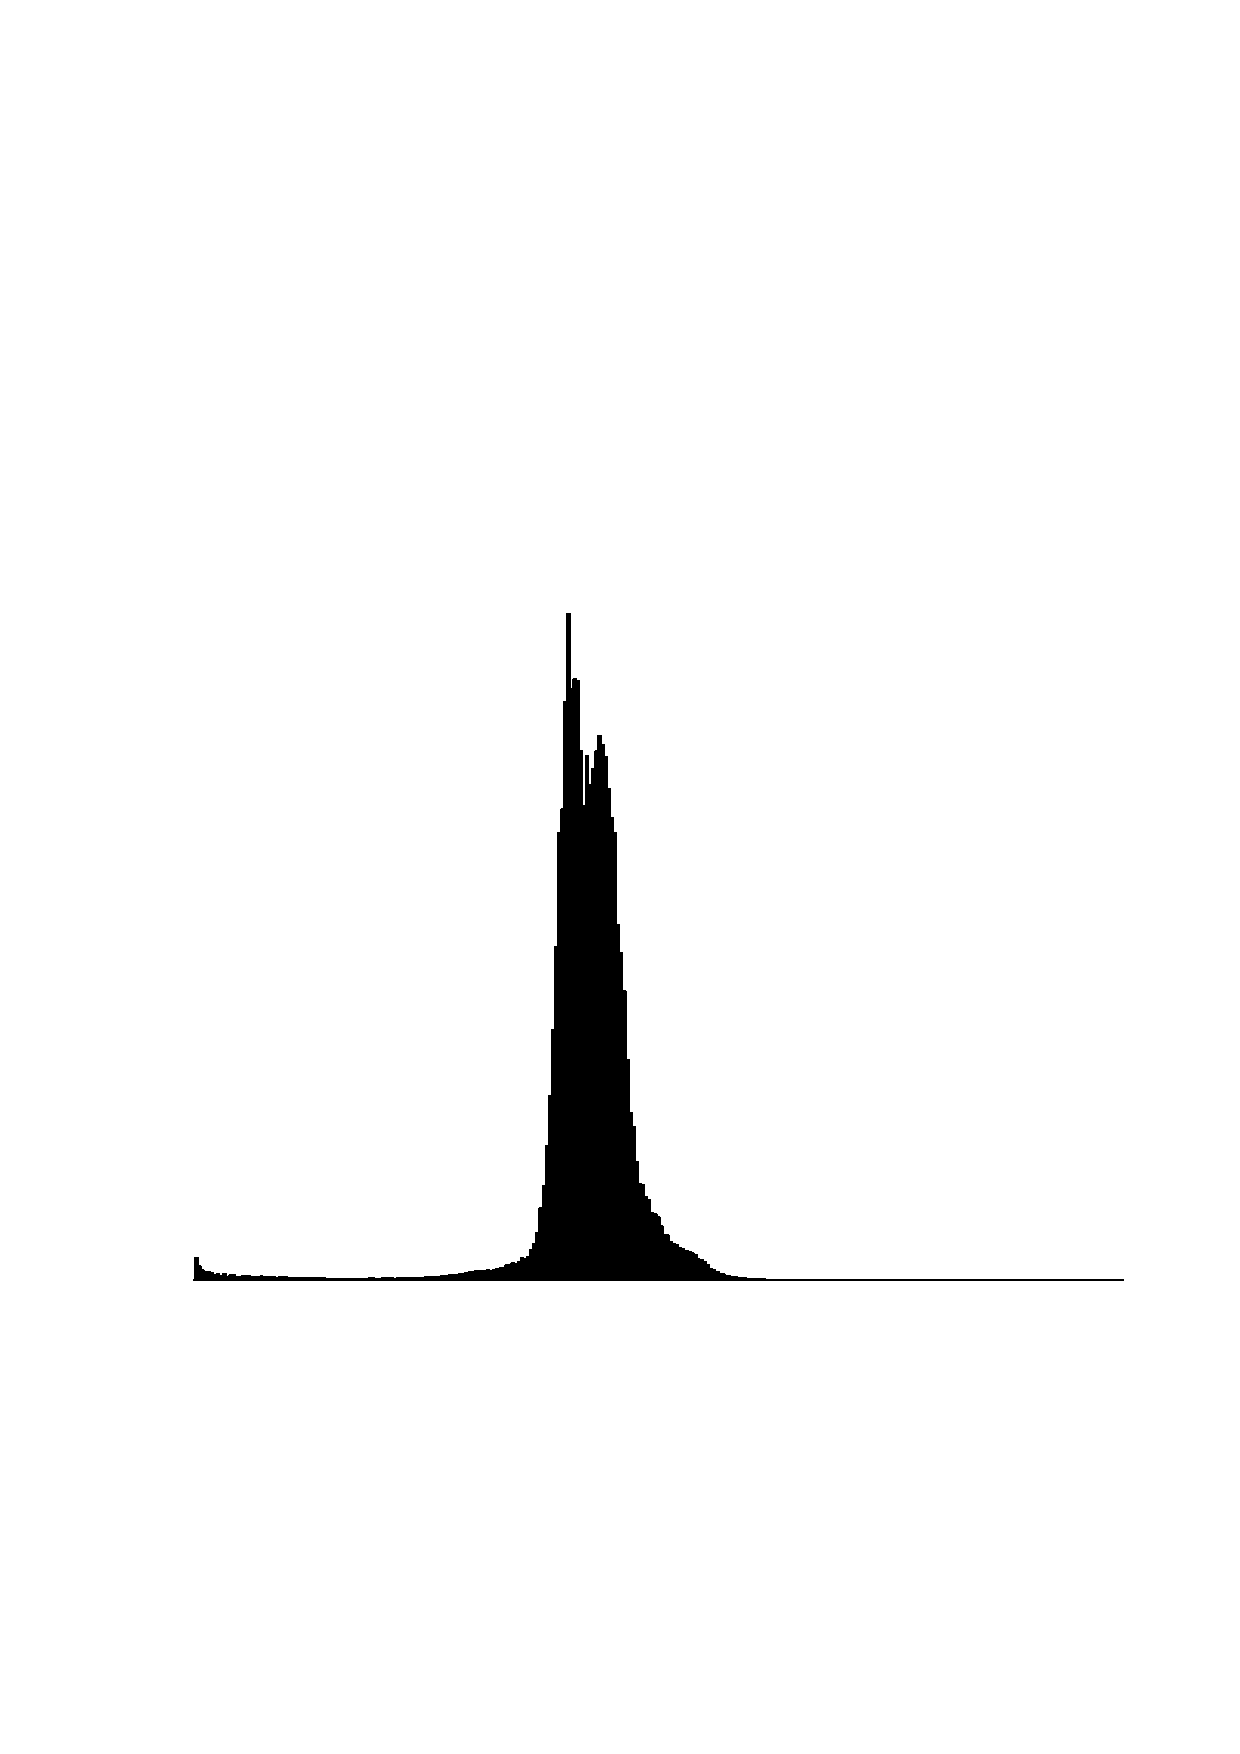
\includegraphics[height=36mm]{images/compress/compressed-mammogram-histogram}}
    \hspace{12pt}
    \subfloat[\label{comp:f}]{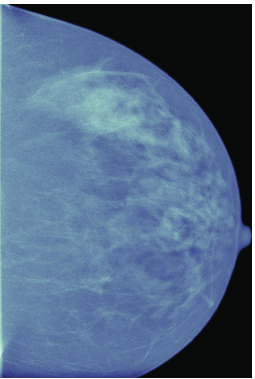
\includegraphics[height=36mm]{images/compress/compressed-mammogram-8bits}}
  \end{center}

  \caption[Conversión de la profundidad de píxeles]
  {Conversión de la profundidad de píxeles. En \protect\subref{comp:e} se
  muestra el histograma generado a partir de la mamografía oscura mostrada en
  \protect\ref{comp:d}, \protect\subref{comp:f} es la imagen de 8 bits
  generada con la función \texttt{imadjust} y \protect\subref{comp:g} es su
  histograma, que es similar al histograma que se muestra en~\ref{comp:b}}.

  \label{img:shrinking-two}
\end{figure}

\subsubsection{Mejoramiento de la imagen.}

Finalmente, ejecutamos un proceso de normalización. El objetivo de este paso es
mejorar la calidad de la imagen que se obtuvo en el paso anterior.

%\definecolor{bg}{rgb}{0.9,0.9,0.9}
%\begin{minted}[linenos=true,
%               fontfamily=fi4,
%               fontseries=ubx,
%               samepage=false,
%               bgcolor=bg]{matlab}
%
%[height width] = size(image);
%imageCopy = repmat(uint8(0), height, width);
%divider = 0.0;
%maxLevel = double(usedGrayLevels);
%while 1
%    divider = divider + 0.01;
%    if maxLevel/divider <= 255
%        break;
%    end
%end
%for h=1:1:height
%    for w=1:1:width
%       imageCopy(h, w) = image(h, w)/divider;
%    end
%end
%\end{minted}

\chapter{Resultados}
\label{resultados}

En este capítulo se exponen las características de la colección de mamografías y
también se aborda una interfaz gráfica de usuario (GUI).

\section{Colección de mamografías}

La colección recibe el nombre \textbf{Colección de Mamografías Digitales
Preprocesadas} (CPDM\footnote{Con el objetivo de que sea accesible a mayor
número de investigadores el nombre oficial de la colección está en inglés:
\textit{Collection of Preprocessed Digital Mammograms}.}. CPDM se constituye
como una fuente de imágenes médicas destinadas al uso de la comunidad
científica. Está disponible públicamente. La colección incluye las mamografías
crudas y las preprocesadas. 

\section{Estructura de CPDM}

La Figura \ref{fig:structure} nos muestra como están organizados los
directorios de la colección. Cada estudio tiene una ficha que contiene datos
del paciente como fecha de nacimiento, fecha del estudio, vista de la imagen,
nombre del archivo y el reporte BIRADS. Cada caso es almacenado en una carpeta,
que contiene la ficha descriptiva y las imágenes con extensión \texttt{.dcm}.
El nombre de cada imagen es la combinación del número de caso más la proyección
correspondiente, por ejemplo, la mama derecha con proyección MLO del primer
caso recibirá el nombre \texttt{0001rmlo.dcm}.

La colección está disponible en la siguiente dirección:
\url{www.casi.dais.mx/cpdm/index.html}. La evaluación de resultados se realizó
utilizando la opinión de los médicos.

\shorthandoff{>} % hack to combine tikZ and Spanish
    \begin{figure}[h]
\begin{center}
\
\tikzstyle{every node}=[draw=black,thick,anchor=west]
\tikzstyle{selected}=[draw=red,fill=red!30]
\tikzstyle{optional}=[dashed,fill=gray!50]

\begin{tikzpicture}[%
  grow via three points={one child at (0.5,-0.7) and
  two children at (0.5,-0.7) and (0.5,-1.4)},
  edge from parent path={(\tikzparentnode.south) |- (\tikzchildnode.west)}]
  \node {servidor}
    child { node [selected] {ftp}
        child { node {código fuente}}
        child { node {imágenes}
            child { node {crudas}
                child { node {caso 1}}
                child { node {...}}
                child { node {caso n}}
            }
            child [missing] {}				
            child [missing] {}				
            child [missing] {}				
            child { node {preprocesadas}
                child { node {caso 1}}
                child { node {...}}
                child { node {caso n}}
            }
        }
    }
    %child [missing] {}				
    child [missing] {}				
    child [missing] {}				
    child [missing] {}				
    child [missing] {}				
    child [missing] {}				
    child [missing] {}				
    child [missing] {}				
    child [missing] {}				
    child [missing] {}				
    child { node [selected] {http}
        child { node {archivos HTML}}
        child { node {archivos CSS}}
    };

\end{tikzpicture}

\end{center}

  \caption[Estructura de CPDM]{Estructura de CPDM}
  \label{fig:structure} 
\end{figure}

\shorthandon{>} 

\section{Interfaz gráfica}

%colormap bone

We built a Graphical User Interface (GUI) system as suggested by  D'Angello
\cite{d2007design}. This GUI allows for mammogram loading and manipulating. 

Following a similar approach as D'Angello \cite{d2007design} as part of the
project it was built a Graphical User Interface (GUI) system who helps the user
to load the mammogram and manipulate it to modify the contrast, increase or
reduce the view. The GUI was developed using Matlab GUIDE. 

De manera similar a D'Angelo \cite{d2007design} se creo una GUI utilizando
Matlab. Como subproducto de este trabajo se creó una interfaz gráfica de
usuario para que los médicos pudiesen modificar los parámetros de la función
CLAHE. Aunque Matlab ofrece un entorno wizard para crear interfaces, escogimos
crear la interfaz a partir de cero debido a las flexibilidades.

La GUI desarrollada tiene un objeto \texttt{uipanel} a la izquierda y un
objecto \texttt{axes} a la derecha (ver Fig. ~\ref{main:before}). El objeto
\texttt{uipanel} contiene la vista previa de las imágenes, allí el usuario
puede elegir cualquiera de las imágenes con un click y en el objeto
\texttt{axes} se visualiza la elección del usuario. 

\begin{figure}[h]
  \begin{center}
    {\includegraphics[height=40mm]{images/gui/main-before}}
  \end{center}
  \caption[GUI: Inicio]{Captura de pantalla de la GUI justo después de inicializar la aplicación} 
  \label{main:before} 
\end{figure}

Se agregó la opción de elegir uno o más archivos para que el usuario tenga la
posibilidad de escoger las diferentes proyecciones en cada caso médico (ver
Fig. ~\ref{fig:openfile}).

\begin{figure}[h]
  \begin{center}
    {\includegraphics[height=40mm]{images/gui/open-file}}
  \end{center}
  \caption[GUI: Selección de archivos]
  {Cuadro de diálogo que permite seleccionar una o más imágenes en formato DICOM} 
  \label{fig:openfile} 
\end{figure}

Se puede navegar en la imagen utilizando las teclas de movimiento o el juego de
teclas \texttt{hjkl} como en los sistemas operativos Unix. En la Fig.
\ref{main:after} se puede apreciar la vista previa de diferentes proyecciones
de una mama en el objeto \texttt{uipanel} y el acercamiento a la imagen en el
objeto \texttt{axes}.

\begin{figure}[h]
  \begin{center}
    {\includegraphics[height=40mm]{images/gui/main-after}}
  \end{center}

  \caption[GUI: Ventana principal 2]{Captura de pantalla de la GUI. A la
  izquierda el componente vertical es el objeto \texttt{uipanel} y a la derecha
  el componente \texttt{axes}} 

  \label{main:after} 
\end{figure}

La mayor parte de las operaciones de preprocesamiento ocurre al momento de
seleccionar y cargar las imágenes. Cuando la imagen está siendo visualizada ya
se ha reducido el área de trabajo, se ha realizado la conversión de bits y se
ha eliminado el ruido. El usuario tiene la posibilidad de mejorar el contraste
de la región visualizada en la sección derecha de la GUI. La interfaz cuenta
con una opción que permite modificar los parámetros de la función que
implementa el algoritmo CLAHE mencionado en la sección anterior (ver
Fig.~\ref{options}). 

Los parámetros modificables por el usuario son \texttt{Tiles by Column} y
\texttt{Tyles by Row}, elementos que establecen el número de divisiones
(mosaicos) de la imagen por columna y renglón respectivamente. \texttt{Contrast
Enhancement Limit}, que específica el valor límite de la mejora del contraste,
\texttt{Number of bins} es el número de columnas del histograma,
\texttt{Distribution} sirve para elegir la forma del histograma y con
\texttt{Range} se precisa el intervalo de los datos de la imagen de salida.

\begin{figure}[h]
  \begin{center}
    {\includegraphics[height=50mm]{images/gui/options}}
  \end{center}
  \caption[GUI: Modificación de parámetros]
  {Ventana que nos permite modificar los valores de entrada de la función CLAHE} 
  \label{options} 
\end{figure}

\section{Retroalimentación médica}

En las primeras pruebas sólo se mejoró  la visualización del tejido graso y no
del tejido mamario.

% consideraciones finales o enviar a conclusión

El código fuente que se generó está disponible en línea bajo un controlador de
versiones en el repositorio: \url{github.com/omartrinidad/mammograms}.


\chapter{Conclusiones}
\label{conclusiones}

Encontramos que 

\section{Trabajos futuros}

Es posible hacer uso de algoritmos más efectivos para la eliminación del ruido y
la mejora del contraste. 

Trabajos similares al nuestro \cite{heath2000digital} han construido cosas como
un servicio web.

El rango de aplicaciones médicas es amplio. El dataset está listo para usarse
en etapas posteriores o ampliar la etapa de procesamiento.

Es posible crear un servicio web [referencia] que recupere las imágenes de
forma efectiva (selección de casos), con una interfaz web responsiva.
Previsualización. de estos casos.

Rescaling. Pasar de una resolución a otra sin problemas.

Preprocesamiento: eliminar el pectoral en las imágenes ¿cranio caudal?
Hacer que las imágenes queden en una sola dirección.

Eliminar el ruido cuántico, algunos trabajos que hablan sobre eso son ... el de
Santos y el de Elsevier

Remover el músculo pectoral en vistas MLO como parte del preprocesamiento.

Proteger la privacidad de los pacientes eliminando el nombre, pero también evitar
que se repitan los casos.


% bibliography APA style
\bibliographystyle{apalike} 
\bibliography{thesis}

\end{document}
